%%
%% Author: Thomas Schouten
%% 23-5-2018
%%

\documentclass[border=5mm, tikz]{standalone}

\usepackage{tikz}

\usetikzlibrary{arrows.meta, decorations.markings}

% Document
\begin{document}

    % Note: for plotting normal functions like y=x**2, use pgfplots instead.

    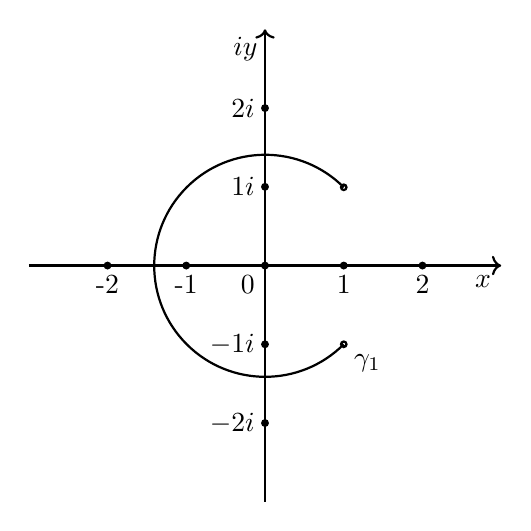
\begin{tikzpicture}[thick]
        % Axes:
        \draw [->] (-3,0) -- (3,0) node [below left]  {$x$};
        \draw [->] (0,-3) -- (0,3) node [below left = -1pt] {$iy$};

        % Axes labels:
        \foreach \n in {-2,-1,1,2}{%
        \draw[fill] (0,\n) circle (1pt) node [left] {$\n i$};
        }
        \foreach \n in {-2,-1,1,2}{%
        \draw[fill] (\n,0) circle (1pt) node [below] {\n};
        }
        \draw[fill] (0,0) circle (1pt) node [below left] {0};

        % Contour line
        \draw (1,-1) circle (1pt) node [below right] {$\gamma_1$} arc (315:45:1.41) circle (1pt);

    \end{tikzpicture}

%    \begin{tikzpicture}[thick, decoration = {
%    %        pre length=2pt,
%    %        post length=2pt,
%    markings,
%    mark=at position 0.7*\pgfdecoratedpathlength with {\arrow {Latex[length=2mm,width=2mm]} }
%    }]
%        % Axes:
%        \draw [->] (-3,0) -- (3,0) node [below left]  {$x$};
%        \draw [->] (0,-3) -- (0,3) node [below left = -1pt] {$iy$};
%
%        % Axes labels:
%        \foreach \n in {-2,-1,1,2}{%
%        \draw[fill] (0,\n) circle (1pt) node [left] {$\n i$};
%        }
%        \foreach \n in {-2,-1,1,2}{%
%        \draw[fill] (\n,0) circle (1pt) node [below] {\n};
%        }
%        \draw[fill] (0,0) circle (1pt) node [below left] {0};
%
%        % Contour line
%        \draw[postaction=decorate] (1,-1) circle (1pt) node [below right] {$\gamma_1$} arc (-45:45:1.41) circle (1pt);
%
%    \end{tikzpicture}

\end{document}